\documentclass[10pt,titlepage]{article}

\usepackage{amsmath}
\usepackage{enumitem}
\usepackage[utf8]{inputenc}
\usepackage[colorlinks,linkcolor=black]{hyperref}
\usepackage{float}
\usepackage{geometry}
\usepackage{graphicx}
\usepackage{listings}
\usepackage{multirow}
\usepackage{parskip}
\usepackage{xcolor}

\geometry{
 a4paper,
 top=25mm,
 bottom=25mm,
}

\restylefloat{table}

\definecolor{codegreen}{rgb}{0,0.6,0}
\definecolor{codegray}{rgb}{0.5,0.5,0.5}
\definecolor{codepurple}{rgb}{0.58,0,0.82}
\definecolor{backcolour}{rgb}{0.95,0.95,0.92}

\lstdefinestyle{mystyle}{
    backgroundcolor=\color{backcolour},
    commentstyle=\color{codegreen},
    keywordstyle=\color{magenta},
    numberstyle=\tiny\color{codegray},
    stringstyle=\color{codepurple},
    basicstyle=\ttfamily\footnotesize,
    breakatwhitespace=false,
    breaklines=true,
    captionpos=b,
    keepspaces=true,
    numbers=left,
    numbersep=1pt,
    showspaces=false,
    showstringspaces=false,
    showtabs=false,
    tabsize=2
}
\lstset{style=mystyle}


\newcommand{\HRule}{\rule{\linewidth}{0.5mm}}
\title{
    \textsc{\LARGE National University of Singapore}\\[1cm]
    \textsc{\Large DSA5104: Group 29}\\[2cm]


    \HRule\\[0.4cm]
    \huge{Comparative Analysis of ``MiniMovieDB" implementations in MySQL, Neo4j and MongoDB}
    \HRule\\[1.5cm]
}

\author{\begin{tabular}{rl}
        Ng Wei Xiang & \\
        Rahul Venkatesh & \\
        Wang YiChen & \\
        Yong Zhu Cheng & 
\end{tabular}}
\date{\vfill\today}

\begin{document}
\maketitle
\tableofcontents
\pagebreak

\section{Introduction}
Through this project, we aim to simulate database development for a complex business problem with a degree of realism
and rigour. Specifically, we challenged ourselves to support the diverse data needs of our chosen client -- a video
streaming service -- and modelled our solution with MySQL, MongoDB and Neo4j systems. We present our overall methodology
and findings below.

\subsection{Project: MiniMovieDB}

We aim to simulate a database system that supports essential product and analysis needs for a hypothetical video
streaming service like Netflix, Disney+ and Prime Video. The key use cases are as follows.

\begin{itemize}
    \item \textbf{Catalogue: Search and Filter} \\
        Users might want to search shows of a specific genre or featuring specific actors. They may want to know what the
        movie is about or who made the soundtrack for it.
    \item \textbf{Recommender System: Explore} \\
        Users might want to try out new shows similar to those they have enjoyed (show-based recommendation). They might
        want to know what other shows they might enjoy based on the similarity in taste with other users (user-based
        recommendation).
    \item \textbf{User Lists} \\
        Users might want to keep track (list) of the shows they have watched or plan to watch, and what they thought
        about a show (rating); similar to \href{https://mydramalist.com/}{MyDramaList}.
    \item \textbf{Business reporting and production planning} \\
        Inventory planning, user behavior analysis.
\end{itemize}

\section{Data Collection}
\subsection{Requirements}
Our data needs to support the analysis of user preferences based on show information and user activity. As such, we
require:
\begin{itemize}
  \item A dataset that provides a wide range of TV shows along with relevant metadata.
  \item A dataset that provides information about user activity, preferences and other relevant details.
\end{itemize}

As detailed user information is difficult to obtain online, we instead focus on anonymized user activity,
where apt and permissible.

Additionally, we require that the datasets:
\begin{itemize}
  \item Have sufficient volume and complexity.
  \item Have sufficient attributes for rich analysis.
  \item Allow linkages between movie information and user data.
\end{itemize}

\subsection{Datasets}
We chose the following datasets for this project.
\begin{itemize}
    \item \href{https://developer.imdb.com/non-commercial-datasets/}{IMDb Non-Commercial Dataset}

        A list of shows and movies with a wide range of features, ranging from basic information (like title, release year
        and runtime) to metadata (like genres, plot and aliases) and cast \& crew.
    \item \href{https://grouplens.org/datasets/movielens/25m/}{MovieLens 25M Dataset}

        Historical records of tagging and rating activity by users (anonymized), with genre information and analysis of
        tag relevance.
\end{itemize}

\subsection{Data Generation}
To further enrich the above datasets, we generate two additional datasets.

\begin{itemize}
    \item Plots, taglines and budget: generated by \href{https://cinemagoer.github.io/}{Cinemagoer} API, a Python package
        for retrieving data from the IMDb movie database.

        This information is valuable in multiple ways. For example, the recommender system can make use of plot information for better recommendations. Plot and tagline information can also be used to support fuzzy search based on user descriptions. For example: ``A show about time
        travel where the protagonist keeps trying to change things but it keeps getting worse."

        \begin{table}[H]
            \centering
            \begin{tabular}{p{0.2\linewidth} | p{0.2\linewidth} | p{0.4\linewidth}}
                \hline
                \textbf{Attribute} & \textbf{Data Type}  & \textbf{Definition}\\
                \hline
                imdbId & string & unique alphanumeric identifier of a show. Consistent with ``tconst" in the IMDb dataset. \\
                \hline
                plot & string & summary of show plot \\
                \hline
                taglines & array & tagline of show \\
                \hline
                budgetAmount & integer & budget of show \\
                \hline
                budgetCurrency & string & currency symbol of show budget \\
                \hline
            \end{tabular}
            \caption{Cinemagoer dataset}
            \label{tab:cinemagoer}
        \end{table}

    \item User Events dataset: Synthetic dataset with simulated user events from impression to rating and tagging.

        User behaviour is a critical vector of analysis for the business, as user conversion, engagement and retention
        are key product and business objectives. This data is often analysed in conjunction with show information for
        important product insights. For convenience, we have used the rating and tagging records from the MovieLens
        dataset as a logical basis for event generation, while also merging them with our synthetic events for a
        comprehensive event log.

        To efficiently generate a dataset with some degree of realism, while keeping the data size manageable, we observe the following principles and considerations in our
        logic.

        \begin{itemize}
            \item Our \textbf{userbase} is the set of users in the MovieLens dataset.

            \item Our event log is based on a \textbf{simplified user journey}, whereby users open the app $\rightarrow$
                scroll through various thumbnails on the home or search page $\rightarrow$ click on the shows that may
                interest them $\rightarrow$ view the corresponding information pop-ups $\rightarrow$ and finally watch a
                show. As such, we have impressions, clicks, views and playbacks as the main event types, with their
                respective probabilities set as:

                $$P(impression) > P(click) > P(view) > P(playback)$$

                (Note that the probabilities in the code are conditional probabilities of each event type on the
                previous. Imposing a descending order on these values is an even stricter condition that helps enlarge
                the difference between event types, to increase the realism of the sample.)
            \item To further mimic an actual event log, we grouped successive events together at random to form 
                \textbf{complete user sessions}.

            \item To \textbf{limit data size}, we restrict the shows that users have interacted with to the shows they have
                tagged and/or rated.

            \item Furthermore, some \textbf{constraints} are in place for basic logical coherence, including:

                \begin{itemize}
                    \item No two distinct user events of a user can overlap chronologically, such as when the
                        \texttt{playbackEndTimestamp} of a previous playback event is greater than the timestamp of the
                        current impression event for the same user.
                    \item The four event types, if present, must take place before a user has tagged or rated the show
                        user.
                \end{itemize}
        \end{itemize}

\end{itemize}

\begin{table}[ht]
    \centering
    \begin{tabular}{p{0.25\linewidth} | p{0.15\linewidth} | p{0.5\linewidth}}
        \hline
        \textbf{Attribute} & \textbf{Data Type} & \textbf{Definition}\\
        \hline
        eventId & string & unique identifier of an event. An event is a single activity performed by a user. \\
        \hline
        sessionId & string & unique identifier of a session. A session is a sequence of events that happened in succession for one user. For example, a user may enter Netflix, scroll through a few movie options, and then watch one to completion. This constitutes one session. \\
        \hline
        userId & integer & unique identifier of a user \\
        \hline
        imdbId & string & unique alphanumeric identifier of a show \\
        \hline
        eventType & string & Type of event. Event types include:
        \textbf{1-impression} (when a page element, e.g. a movie thumbnail, is visible to a user),
        \textbf{2-click} (when a user clicks on any page element, e.g. a movie card),
        \textbf{3-view} (when a user views the opened page element, i.e. a movie info pop-up),
        \textbf{4-playback} (when a user watches a show),
        \textbf{5-rate} (as per MovieLens),
        \textbf{6-tag} (as per MovieLens) \\
        \hline
        timestamp & integer & UTC timestamp of event. Timestamps for rating and tagging events are from the
        MovieLens dataset \\
        \hline
        playbackEndTimestamp & integer & The time at which a user stops a show \\
        \hline
        rating & float & The rating given by the user. Made on a 5-star scale with half-star increments. Taken
        from the MovieLens dataset \\
        \hline
        tag & string & user-generated metadata about the movie. Taken from the MovieLens dataset \\
        \hline
    \end{tabular}
    \caption{User Events dataset}
    \label{tab:user_events}
\end{table}

Professionally, event logs are a much more complicated business. As such, we note that many details have
indeed been omitted or simplified for the project. For example, session definitions are usually more precise (e.g., a
session ends only when a user has been inactive for a certain amount of time). Many edge cases in user behaviour have
not been accounted for (e.g., when users pause and play the same show multiple times) and tracked event types are in
fact much more diverse than the above four.

\pagebreak

\begin{center}
\begin{figure}[H]
    \centering
    \includegraphics[scale=0.8]{event_dist.png}
    \caption{Event Distribution}
    \label{fig:event_dist}

    \hspace*{-2cm}\includegraphics[scale=0.5]{user_event_dist.png}
    \caption{User Activity Distribution}
    \label{fig:user_event_dist}
\end{figure}
\end{center}

We note that the event distribution of the dataset is consistent with our design, whereby impression, click, view and
playback events occur in decreasing order of frequency. We further note that user activity skews left significantly,
with almost all users generating total event counts below 2000 each.


\section{Understanding our data}

\subsection{IMDb non-Commercial dataset}
\begin{itemize}
    \item Shows (title.basics.tsv.gz): essential information about all shows covered by this dataset

        \begin{table}[H]
            \centering
            \begin{tabular}{p{0.2\linewidth} | p{0.2\linewidth} | p{0.4\linewidth}}
                \hline
                \textbf{Attribute} & \textbf{Data Type}  & \textbf{Definition}\\
                \hline
                tconst & string & an alphanumeric unique identifier of the title \\
                \hline
                titleType & string & the type/format of the title (e.g. movie, short,  tvseries, tvepisode, video, etc) \\
                \hline
                primaryTitle & string & the more popular title / the title used by the  filmmakers on promotional
                materials at the point of  release \\
                \hline
                originalTitle & string & original title, in the original language \\
                \hline
                isAdult & integer & 0: non-adult title; 1: adult title \\
                \hline
                startYear & integer & release year of a title. In the case  of TV Series, it is the
                series start year \\
                \hline
                endYear & integer & TV Series end year. 'W' for all other title types \\
                \hline
                runtimeMinutes & integer & runtime of the title in minutes \\
                \hline
                genres & array & includes up to three genres associated with the title \\
                \hline
            \end{tabular}
            \caption{title.basics.tsv}
            \label{tab:imdb_basics}
        \end{table}

    \item Alternative Titles (title.akas.tsv.gz): in different languages and regions

        \begin{table}[H]
            \centering
            \begin{tabular}{p{0.2\linewidth} | p{0.2\linewidth} | p{0.4\linewidth}}
                \hline
                \textbf{Attribute} & \textbf{Data Type}  & \textbf{Definition}\\
                \hline
                titleId & string & an alphanumeric unique identifier of the title, i.e. tconst \\
                \hline
                ordering & integer & a number to uniquely identify rows for a given titleId \\
                \hline
                title & string & the localized title \\
                \hline
                region & string & the region for this version of the title \\
                \hline
                language & string & the language of the title \\
                \hline
                types & array & Enumerated set of attributes for this alternative title. One or more of the following:
                ``alternative", ``dvd",  ``festival", ``tv", ``video", ``working", ``original",  ``imdbDisplay". New values may
                be added in the  future without warning \\
                \hline
                attributes & array & Additional terms to describe this alternative title, not  enumerated \\
                \hline
                is OriginalTitle & integer & 0: not original title; 1: original title \\
                \hline
            \end{tabular}
            \caption{title.akas.tsv}
            \label{tab:imdb_akas}
        \end{table}

    \item Crew (title.crew.tsv.gz): director(s) and writer(s)

        \begin{table}[H]
            \centering
            \begin{tabular}{p{0.2\linewidth} | p{0.2\linewidth} | p{0.4\linewidth}}
                \hline
                \textbf{Attribute} & \textbf{Data Type}  & \textbf{Definition}\\
                \hline
                tconst & string & an alphanumeric unique identifier of the title \\
                \hline
                directors & array & director(s) of the given title \\
                \hline
                writers & array & writer(s) of the given title \\
                \hline
            \end{tabular}
            \caption{title.crew.tsv}
            \label{tab:imdb_crew}
        \end{table}

    \item Episode (title.episode.tsv.gz)

        \begin{table}[H]
            \centering
            \begin{tabular}{p{0.2\linewidth} | p{0.2\linewidth} | p{0.4\linewidth}}
                \hline
                \textbf{Attribute} & \textbf{Data Type}  & \textbf{Definition}\\
                \hline
                tconst & string & an alphanumeric unique identifier of the episode \\
                \hline
                parentTconst & string & alphanumeric identifier of the parent TV Series \\
                \hline
                seasonNumber & integer & season number the episode belongs to \\
                \hline
                episodeNumber & integer & episode number of the tconst in the TV series \\
                \hline
            \end{tabular}
            \caption{title.episode.tsv}
            \label{tab:imdb_episode}
        \end{table}

    \item Ratings (title.ratings.tsv.gz)

        \begin{table}[H]
            \centering
            \begin{tabular}{p{0.2\linewidth} | p{0.2\linewidth} | p{0.4\linewidth}}
                \hline
                \textbf{Attribute} & \textbf{Data Type}  & \textbf{Definition}\\
                \hline
                tconst & string & an alphanumeric unique identifier of the title \\
                \hline
                averageRating & float & weighted average of all the individual user ratings \\
                \hline
                numVotes & integer & number of votes the title has received \\
                \hline
            \end{tabular}
            \caption{title.ratings.tsv}
            \label{tab:imdb_ratings}
        \end{table}

    \item Principals (title.principals.tsv.gz): key personnel involved in the making of a show

        \begin{table}[H]
            \centering
            \begin{tabular}{p{0.2\linewidth} | p{0.2\linewidth} | p{0.4\linewidth}}
                \hline
                \textbf{Attribute} & \textbf{Data Type}  & \textbf{Definition}\\

                \hline
                tconst & string & an alphanumeric unique identifier of the title \\
                \hline
                ordering & integer & a number to uniquely identify rows for a given titleId \\
                \hline
                nconst & string & alphanumeric unique identifier of the name/person \\
                \hline
                category & string & the category of job that person was in \\
                \hline
                job & string & the specific job title if applicable, else 'IN' \\
                \hline
                characters & arrays & the names of the characters played if applicable, else 'IN' \\

                \hline
            \end{tabular}
            \caption{title.principals.tsv}
            \label{tab:imdb_principals}
        \end{table}

    \item People (name.basics.tsv.gz): information about the real person

        \begin{table}[H]
            \centering
            \begin{tabular}{p{0.2\linewidth} | p{0.2\linewidth} | p{0.4\linewidth}}
                \hline
                \textbf{Attribute} & \textbf{Data Type}  & \textbf{Definition}\\


                \hline
                nconst & string & an alphanumeric unique identifier of the name/person \\
                \hline
                primaryName & string & name by which the person is most often credited \\
                \hline
                birthYear & integer & in YYYY format \\
                \hline
                deathYear & integer & in YYYY format if applicable, else 'IN' \\
                \hline
                primaryProfession & array & the top 3 professions of the person \\
                \hline
                knownforTitles & array & titles the person is known for \\
                \hline

                \hline
            \end{tabular}
            \caption{names.basics.tsv}
            \label{tab:imdb_names}
        \end{table}
\end{itemize}


\pagebreak
\subsection{MovieLens dataset}
\begin{itemize}
    \item Ratings (ratings.csv)

        \begin{table}[H]
            \centering
            \begin{tabular}{p{0.2\linewidth} | p{0.2\linewidth} | p{0.4\linewidth}}
                \hline
                \textbf{Attribute} & \textbf{Data Type}  & \textbf{Definition}\\
                \hline
                userId & integer & an alphanumeric unique identifier of a user \\
                \hline
                movieId & integer & a unique identifier of a movie, as set by MovieLens \\
                \hline
                rating & float & rating given by user. Made on a 5-star scale with half-star increments \\
                \hline
                timestamp & integer & Timestamp of rating record. Represents seconds since midnight of January 1, 1970
                in UTC time \\
                \hline
            \end{tabular}
            \caption{ratings.csv}
            \label{tab:ml_ratings}
        \end{table}

    \item Tags (tags.csv): user-generated metadata about movies. Each tag is typically a single word or short phrase. The
        meaning, value, and purpose of a particular tag is determined by each user. Example: ``alien", ``surreal",
        ``justice".

        \begin{table}[H]
            \centering
            \begin{tabular}{p{0.2\linewidth} | p{0.2\linewidth} | p{0.4\linewidth}}
                \hline
                \textbf{Attribute} & \textbf{Data Type}  & \textbf{Definition}\\

                \hline
                userId & integer & an alphanumeric unique identifier of a user \\
                \hline
                movieId & integer & a unique identifier of a movie, as set by MovieLens \\
                \hline
                tag & string & user-generated metadata about the movie. The meaning, value and purpose of a tag is determined by each user. A user can cast multiple tags \\
                \hline
                timestamp & integer & Timestamp of tagging record. Represents seconds since midnight of January 1, 1970 in UTC time \\
                \hline

            \end{tabular}

            \caption{tags.csv}
            \label{tab:ml_tags}
        \end{table}

    \item Movies (movies.csv): genre information

        \begin{table}[H]
            \centering
            \begin{tabular}{p{0.2\linewidth} | p{0.2\linewidth} | p{0.4\linewidth}}
                \hline
                \textbf{Attribute} & \textbf{Data Type}  & \textbf{Definition}\\

                \hline
                movieId & integer & a unique identifier of a movie, as set by MovieLens \\
                \hline
                title & string & title of movie. Includes release year in parentheses at the end of the title \\
                \hline
                genre & string & pipe-separated list of genres that best characterize the movie \\
                \hline
            \end{tabular}

            \caption{movies.csv}
            \label{tab:ml_movies}
        \end{table}

    \item Links (links.csv): links MovieLens id to IMDb id and TMDb id for a show.

        \begin{table}[H]
            \centering
            \begin{tabular}{p{0.2\linewidth} | p{0.2\linewidth} | p{0.4\linewidth}}
                \hline
                \textbf{Attribute} & \textbf{Data Type}  & \textbf{Definition}\\

                \hline
                movieId & integer & a unique identifier of a movie, as set by MovieLens \\
                \hline
                imdbId & string & a unique alphanumeric identifier of the movie, as set by IMDb. Corresponds to tconst
                \\
                \hline
                tmdbId & string & a unique identifier of the movie, as set by themoviedb.org. Note that this identifier, while available
                in the raw data, is not used for any purposes in this project \\
                \hline


            \end{tabular}
            \caption{links.csv}
            \label{tab:ml_links}
        \end{table}

    \item Tag Genome (genome-tags.csv): tag genome IDs

        \begin{table}[H]
            \centering
            \begin{tabular}{p{0.2\linewidth} | p{0.2\linewidth} | p{0.4\linewidth}}
                \hline
                \textbf{Attribute} & \textbf{Data Type}  & \textbf{Definition}\\

                \hline
                tagId & integer & a unique identifier of the genome tag assigned to the movie \\
                \hline
                tag & string & the actual genome tag assigned \\
                \hline

            \end{tabular}
            \caption{genome-tags.csv}
            \label{tab:ml_genome_tags}
        \end{table}

    \item Tag Genome Scores (genome-scores.csv): Relevance scores of a tag genome to a show. The tag genome encodes how
        strongly movies exhibit particular properties represented by tags.

        \begin{table}[H]
            \centering
            \begin{tabular}{p{0.2\linewidth} | p{0.2\linewidth} | p{0.4\linewidth}}
                \hline
                \textbf{Attribute} & \textbf{Data Type}  & \textbf{Definition}\\

                \hline
                movieId & integer & a unique identifier of a movie, as set by MovieLens \\
                \hline
                tagId & integer & a unique identifier of the tag assigned to the movie.  tagId values are generated when the data set is
                exported, and thus vary from version to version of  this dataset  Note that the tags here are a subset of the tags
                recorded in tags.csv, and are henceforth referred to  as ``genome tags" \\
                \hline
                relevance & float & Relevance score of genome tag \\
                \hline

            \end{tabular}
            \caption{genome-scores.csv}
            \label{tab:ml_genome_scores}
        \end{table}


\end{itemize}

\pagebreak
\subsection{Summary Statistics}

\begin{itemize}
\item \textbf{IMDb non-commercial dataset}

\begin{center}
\begin{tabular}{l|r|r|l}
\hline
\textbf{Domain} & \textbf{Size} & \textbf{Volume (len)} & \textbf{Comments} \\
\hline
Shows & $841 \mathrm{MB}$ & 10\,274\,873 & startYear range: $1874-2031$ \\
\hline
Alternative Titles & $1.8 \mathrm{GB}$ & 37\,595\,404 &  \\
\hline
Crew & $324 \mathrm{MB}$ & 10\,275\,873 &  \\
\hline
Episodes & $195 \mathrm{MB}$ & 7\,835\,881 &  \\
\hline
Ratings & $23 \mathrm{MB}$ & 1\,364\,343 &  \\
\hline
Principals & $2.5 \mathrm{GB}$ & 58\,856\,068 &  \\
\hline
People & 753MB & 12\,969\,698 &  \\
\hline
\end{tabular}
\end{center}


\item \textbf{MovieLens dataset}

\begin{center}
\begin{tabular}{l|r|r|l}
\hline
\textbf{Domain} & \textbf{Size} & \textbf{Volume (len)} & \textbf{Comments} \\
\hline
Ratings & $662 \mathrm{MB}$ & 25\,000\,095 & \begin{tabular}{l}
User count: 162\,541 \\
Date range: \\
1995-01-09 to 2019-11-21 \\
\end{tabular} \\
\hline
Tags & $38 \mathrm{MB}$ & 1\,093\,360 & \begin{tabular}{l}
User count: 14\,592 \\
Date range: \\
2005-12-24 to 2019-11-21 \\
\end{tabular} \\
\hline
Movies & $3 \mathrm{MB}$ & 62\,423 &  \\
\hline
Links & $1 \mathrm{MB}$ & 62\,423 &  \\
\hline
Tag Genome & $18 \mathrm{~KB}$ & 1128 &  \\
\hline
Tag Genome Scores & $425 \mathrm{MB}$ & 15\,584\,448 &  \\
\hline
\end{tabular}
\end{center}

\item \textbf{Generated datasets}

\begin{center}
\begin{tabular}{l|r|r|l}
\hline
\textbf{Domain} & \textbf{Size} & \textbf{Volume (len)} & \textbf{Comments}\\
\hline
Cinemagoer & $20 \mathrm{MB}$ & 62\,420 \\
\hline
User Events & 4.12GB & 72\,870\,860 & \begin{tabular}{l}
User count: 162\,541 \\
Date range: \\
1995-01-03 to 2019-11-21 \\
\end{tabular} \\
\hline
\end{tabular}
\end{center}

\end{itemize}


\newpage
\section{Data Processing and Cleaning}
Different databases have different pre-processing needs. Here, we highlight the common processes. Pre-processing for
MongoDB is covered under that section.

\subsection{Processing Timestamps}
All timestamp values of user events have been cast in UTC time and presented in the ISO format: yyyy-mm-dd hh-mm-ss.

MongoDB stores timestamps as integers to save space, specifically in User Events where timestamps are not typically
displayed to the user. For user ratings, however, timestamp can be converted to \texttt{ISODate}.

\subsection{Processing Arrays}
There are multiple fields in the IMDb dataset with array values, such as genres, directors and writers. As they are each
formatted differently in the raw data, we have processed these fields to accommodate the following cases:

\begin{itemize}
  \item Arrays formatted as strings delimited by `$\mathrm{x}02$'

  \item Arrays formatted as strings delimited by `,'. Specifically, some fields use double inverted commas for array
      elements while others use single inverted commas.

  \item Arrays formatted as strings delimited by `$\mid$'.
\end{itemize}

\subsection{Remove Placeholder Titles}
In the IMDb dataset, many titles of TV show episodes have been written as ``Episode \\
\#\{seasonNumber\}.\{episodeNumber\}". This information is already captured by other attributes, thus the title does not
add any new information. This also leads to unrelated TV shows to have identical titles, which can be confusing.
As such, we removed such values from the ``primaryTitle" and ``originalTitle" fields. (MongoDB retains these.)

\subsection{Standardize Identifiers}
The \texttt{imdbId} values in the MovieLens dataset do not have the prefix ``tt" found in the IMDb dataset. We prefix them to form \texttt{ttxxxxxxx}.

\subsection{Standardize Semantics}
We standardized overlapping field names based on the following conventions, mostly for clarity and interpretability. For
example, 'titles' is replaced by 'shows', while the ratings field in the IMDb dataset is prefixed with 'imdb':

\begin{center}
\begin{tabular}{|l|l|}
\hline
Standardized Field Name & Original Field Name(s) \\
\hline
imdbId & \begin{tabular}{l}
- tconst \\
- parentTconst \\
- titleId \\
- imdbId (links.csv)\\
\end{tabular} \\
\hline
showType & genres (title.basics.tsv.gz) \\
\hline
aliasTypes & types (title.akas.tsv.gz) \\
\hline
personId & nconst \\
\hline
knownForShows & knownforTitles (name.basics.tsv.gz) \\
\hline
imdbAvgRating & averageRating (title.ratings.tsv.gz) \\
\hline
genomeTagId &  tagId (genome-tags.csv, genome-scores.csv)\\
\hline
genomeTag & tag (genome-tags.csv) \\
\hline
\end{tabular}
\end{center}

\section{Data Storage}

\subsection{MySQL: Document Database}
\subsubsection{Schema}
\begin{figure}[H]
    \hspace*{-2cm}\includegraphics[width=1.25\textwidth]{mysql_er.png}
    \caption{Conceptual Design: ER Diagram}
    \label{fig:mysql_er}
\end{figure}

\begin{center}
    \begin{figure}[H]
        \centering
        \hspace*{-2cm}\includegraphics[width=1.25\textwidth]{mysql_schema_new.png}
        \caption{Logical Design: Schema Diagram}
        \label{fig:mysql_schema}
    \end{figure}
\end{center}

\subsubsection{BCNF Discussion}

We made multiple schema refinements to remove unwanted functional dependencies (FD) from the relations concerned. For
example, \texttt{user\_id} was removed from the \texttt{event} (merged with
\texttt{event\_user}) relation, due to the \texttt{sessionId} $\rightarrow$ \texttt{userId} FD. As such, there are
presently no relations in our schema that carry non-trivial FDs beyond their candidate keys.

We further note that by the union principle, most of these decompositions havebeen dependency-preserving. However, with separation of the rating, tag and endTimeStamp attributes due to the large amount of null values (as discussed later), the rating $\rightarrow$ eventType, tag $\rightarrow$ eventType and endTimeStamp $\rightarrow$ eventType FDs could not be preserved.

\subsubsection{Trade-off between Storage Efficiency and Query Speed}
When designing our schema, we needed to also consider the impact of null values, which is pertinent to the `show' and `event' relations. For example, in the former relation, some attributes like imdbAverageRating and endYear contain a lot of null values. Although these attributes can be extracted and split into multiple tables to save space, doing so creates the need for expensive outer joins  in queries, which significantly reduces query speeds. Considering further that the attributes in the show table would be frequently used in queries, we decided to trade storage efficiency for query speed, and store these attributes in one large table. 

As for the events table, certain event types also come with their own distinct attributes, such as tag and rating, which thus contain many null values. However, in this case, the eventType attribute allows us to select specific events to join with separated attributes, ergo our decision to store these attributes separately.



\subsubsection{Advantages and Limitations}
MySQL has a strict predefined schema that requires the structure and type of data to be fixed. It also allows the construction of different types of constraints for each attribute. This protects the data from incorrect input and other mistakes.

However, inflexible schema could also lead to some problems. MYSQL does not support storing arrays in a single column, so a one-to-many relationship would require two separate tables, which have to be joined together for some queries. This could increase query runtimes rather significantly.

\pagebreak
\subsection{MongoDB: Document Database}
\subsubsection{Collections}

\begin{lstlisting}
people
    - name
    - birth
    - death
    - profession
    - knownFor (list shows)
\end{lstlisting}

\begin{lstlisting}
shows
    - primaryTitle
    - startYear
    - endYear
    - runtime
    - isAdult
    - genres (list str)
    - aka (list str)
    - taglines (list str)

    - plot
    - tags (list (str, relevance))

    - actors (list)
        + peopleId
        + character list
    - crew (list)
        + peopleId
        + job

    - averageRating
    - numVotes

    - seasonNumber
    - episodeNumber
    - parentId (show)
\end{lstlisting}
\begin{lstlisting}
user_ratings:
    - userId
    - imdbId
    - rating
    - timestamp
\end{lstlisting}

\begin{lstlisting}
user_events:
    - userId
    - sessionId
    - imdbId
    - eventType
    - timestamp
    - playbackEndTimestamp (for type = playback only)
\end{lstlisting}

Indices:
\begin{lstlisting}
shows.primaryTitle
people.name
user_events.userId
user_events.eventType
user_ratings.userId
user_ratings.imdbId
\end{lstlisting}

\pagebreak
\textbf{Choices and \href{https://www.mongodb.com/developer/products/mongodb/mongodb-schema-design-best-practices/}{best
practices}}:
\begin{itemize}
    \item Notice that our schema (list of collections) is lot less convoluted than the preceding MySQL schema.
        \textbf{No schema hassles} is one of the selling points of MongoDB.
    \item I decide to \textbf{embed} as much as possible. Actors and crew are still referenced, but we can duplicate
        \texttt{people.name} into \texttt{show} \textbf{to avoid lookup} should the need arise.
    \item \texttt{user\_ratings} and \texttt{user\_events} are separate because they are rarely used in conjunction, no
        no lookups.
    \item If our recommender system relies heavily on tags, we can \textbf{create a new collection} \texttt{show\_tags}.
        Tags are indeed basic information that a user would be interested in, but if we can we should \textbf{avoid long
        arrays}.
    \item \texttt{nconst} and \texttt{tconst} are stored in \texttt{\_id} directly rather than a random \texttt{ObjectID}.
    \item Since MongoDB schema is quite tolerant to structural changes, we can \textbf{easily} update the documents to
        \textbf{add more fields} should we want to store more information.
\end{itemize}

\subsubsection{Processing, Importing and Querying}
\begin{itemize}
    \item Bulk import using \texttt{mongoimport} rather than via a programming language like Python.
    \item Read dataset, join and transform into \texttt{csv} for flat structures and \texttt{json} for lists.
    \item Import \texttt{csv} to create the document, then import and merge \texttt{json} with existing documents. This
        ensures your computer won't hang due to memory usage.
    \item In case we want to add more fields, we can import merge the partial documents as mentioned above.
    \item Complex queries are usually carried out as \texttt{aggregates} (pipelines). Instead of joins like in SQL, we
        have lookups.
    \item The code for processing, importing and queries can be found in \href{https://github.com/recurze/MiniMovieDB}{this repository}.

\end{itemize}

\subsubsection{Validation Rules}
\begin{itemize}
    \item Since initial documents are generated, we can apply validation rules during this generation process directly.
    \item For subsequent inserts and updates, we want to set up validation rules in mongodb like:
        \begin{itemize}
            \item All integers are positive
            \item \texttt{birth} $\le$ \texttt{death}; \texttt{startYear} $\le$ \texttt{endYear}
            \item 0 $\le$ \texttt{averageRatings} $\le$ 10; \texttt{rating} on scale of 5 with increments
                of 0.5
        \end{itemize}
\end{itemize}

\subsubsection{Advantages and Limtiations}
Without schemas, data writes and insertions are highly convenient on MongoDB. By accommodating more flexible structures in the form of hierarchies, sub-documents and arrays, MongoDB allows us to store less structured data a lot more quickly, while also speeding up certain types of queries.

On the other hand, we observe high memory usage due to unwinding, lack of joins and duplication. The 16MB size limit on documents may also be problematic if the list of tags grows.


\pagebreak
\subsection{Neo4j: Graph Database}

\subsubsection{Schema}

\begin{center}
    \begin{figure}[H]
        \centering
        \hspace*{-2cm}\includegraphics[width=1.25\textwidth]{neo4j_schema.png}
        \caption{Schema Diagram}
        \label{fig:neo4j_schema}
    \end{figure}
\end{center}

Each table represents a node in the graph, with the header (camel-cased and starting with an uppercase character) denoting the label of the node. The properties of the node are listed as members of the table. For instance, a show would be represented as one node in the graph with the label 'Show'. The count statistics of each node label are as follows:

\begin{center}
\begin{tabular}{l|r|l|r}
\hline
nodeLabel & numberOfNodes & nodeLabel & numberOfNodes \\
\hline
``Show" & $10\,241\,550$ & ``Job" & $58\,593\,659$ \\
\hline
``Alias" & $69\,120\,540$ & ``User" & 162\,541 \\
\hline
``ShowType" & 11 & ``JobCategory" & 12 \\
\hline
``Genre" & 30 & ``Tag" & 73\,050 \\
\hline
``Person" & $12\,923\,154$ & ``Session" & 434\,325 \\
\hline
``AliasType" & 8 & ``GenomeTag" & 1\,128 \\
\hline
``Region" & 247 & ``Event" & $72\,870\,860$ \\
\hline
``Language" & 107 & ``EventType" & 6 \\
\hline
``Profession" & 43 &  &  \\
\hline
\end{tabular}
\end{center}

Each arrow between the two tables represents a directed edge, otherwise known as an arc, between the corresponding nodes. The label of the arc is denoted along the arc in uppercase with an underscore separating the words, with its properties listed in bullet points. For instance, if a show has an alias, it would be represented as an arc from the 'Show' node representing that particular show to the 'Alias' node representing that particular alias. The count statistics of each arc label are as follows:

\begin{center}
\begin{tabular}{l|r|l|r}
\hline
arcLabel & numberOfArcs & arcLabel & numberOfArcs \\
\hline
``IS\_GENRE" & $31\,738\,804$ & ``DID\_JOB" & $117\,187\,318$ \\
\hline
``IS\_SHOW\_TYPE" & $20\,464\,630$ & ``IS\_JOB\_CATEGORY" & $117\,187\,318$ \\
\hline
``AKA" & $74\,967\,224$ & ``HAS\_PROFESSION" & $28\,547\,696$ \\
\hline
``HAS\_ALIAS\_TYPE" & $11\,370\,466$ & ``KNOWN\_FOR\_SHOW" & $42\,497\,188$ \\
\hline
``FROM\_REGION" & $71\,158\,298$ & ``HAS\_GENOME\_TAG" & $31\,168\,896$ \\
\hline
``IN\_LANGUAGE" & $61\,425\,630$ & ``HAS\_SESSION" & 868\,650 \\
\hline
``DIRECTED\_BY" & $15\,570\,102$ & ``HAS\_EVENT" & $145\,741\,720$ \\
\hline
``WRITTEN\_BY" & $24\,635\,724$ & ``INVOLVED\_SHOW" & $145\,741\,720$ \\
\hline
``HAS\_EPISODE" & $15\,600\,236$ & ``IS\_EVENT\_TYPE" & $145\,741\,720$ \\
\hline
``OFFER\_JOB" & $117\,187\,318$ & ``WITH\_TAG" & $2\,186\,688$ \\
\hline
\end{tabular}
\end{center}

Constraints are also added for robustness. The key constraints are added to property or a composite set of properties
for each node type, denoted by an underline. These properties serve as an uniqueness and existence constraints for those
nodes, akin to the primary keys concept in relational databases. For instance, creating a ``Show" node with the same
``imdbId" as another existing ``Show" node would result in an error because the \texttt{imdbId} must be unique across
all ``Show" nodes. Creating a ``Show" node without \texttt{imdbId} would also be rejected as \texttt{imdbId} is not nullable.

\subsubsection{Advantages and Limitations}
Similar to other non-relational databases such as MongoDB as described above, Neo4j does not require the data to be of
the same structure. For instance, for an entity Show, if it does not have some properties such as ``taglines", it would
simply be modelled as \texttt{null}.

Neo4j also offers the flexibility to store arrays as its properties. For instance, if a show has multiple taglines, they could be stored as a property of the show node in an array of strings.

However, the type of constraints available are limited to only uniqueness and/or existence constraints. As such, not all checks
could be performed to ensure data integrity. For instance, creating an event node with an \texttt{endTimestamp} earlier
than its \texttt{timestamp} would not result in an error even though the data does not make sense to have the event
ending before it starts.

\pagebreak
\section{Data Access}

\subsection{Queries}
\textbf{DB Management}
\begin{enumerate}
    \item The company has produced a new show. Add a new show with \texttt{imdbId} ``tt51045104", \texttt{primaryTitle}
        as ``DSA5104 Project", and \texttt{startYear} as 2023.
    \item The company needs to update a show that is ending. Update the show with \texttt{imdbId} ``tt51045104" with
        \texttt{endYear} of 2023.
\end{enumerate}

\textbf{Search}
\begin{enumerate}[resume]
    \item The user would like to search for a show named ``Pulp Fiction." List all shows with primary title containing
        case-insensitive ``pulp fiction" as a substring.

        \textbf{Expected columns:} \texttt{imdbId}, \texttt{primaryTitle}, \texttt{startYear}, \texttt{plot}.

    \item The user forgot the title of the show but remembers a tagline ``may the force be with you". Find the show with
        a tagline containing case-insensitive ``may the force be with you" as a substring.

        \textbf{Expected columns:} \texttt{imdbId}, \texttt{primaryTitle}, \texttt{startYear}, \texttt{plot}.

    \item The user has preferences as shown below. List the shows with at least one of the user’s matching preferences
        for each category.
        \begin{itemize}
            \item Genre: Adventure, Thriller 
            \item Actor/actress: Cillian Murphy, Anne Hathaway 
            \item Director: Quentin Tarantino, Christopher Nolan 
        \end{itemize}

        \textbf{Expected columns:} \texttt{imdbId}, \texttt{primaryTitle}, \texttt{startYear}, \texttt{plot}.

    \item The user would like to indulge in a show with many episodes. Find all the episodes of the show with the
        greatest number of episodes where the episode primary title, season number and episode number are all known, in
        chronological order.

        \textbf{Expected columns:} \texttt{imdbId}, \texttt{primaryTitle}, \texttt{seasonNumber},
        \texttt{episodeNumber}.

    \item The user would like to retrieve its past activities. List all events of the last session of the user with
        userId ``5104" in chronological order.

        \textbf{Expected columns:} \texttt{sessionId}, \texttt{eventId}, \texttt{eventType}, \texttt{imdbId},
        \texttt{timestamp}.
\end{enumerate}

\textbf{Inventory Planning}
\begin{enumerate}[resume]
    \item The company would like to manage its inventory by removing and adding shows. List 10 best and 10 worst shows
        rated at least 100 times, sorted by average rating.

        \textbf{Expected columns:} \texttt{imdbId}, \texttt{primaryTitle}, \texttt{avgRating}, \texttt{numRating}.
\end{enumerate}

\textbf{User Analysis}
\begin{enumerate}[resume]
    \item The company would like to create a dashboard showing the key metrics of user activities. Find the following
        metrics aggregated over all users during week X (only considering events starting from the first impression
        event onwards during week X):
        \begin{align*}
            N &= \text{num of users} \\
            avgNumShows &= \frac{1}{N}\sum_{user} \text{num of distinct shows playback'ed by } user \\
            avgWatchTime &= \frac{1}{N}\sum_{user} \text{total playback duration of all events of } user \\
            avgClickThruRate &= \frac{1}{N}\sum_{user} \frac{\text{num of click events}}{\text{num of impression events}} \\
            avgWatchRate &= \frac{1}{N}\sum_{user} \frac{\text{num of playback events}}{\text{num of click events}} \\
        \end{align*}

    \item The company would like to provide further details of the playback events in the dashboard by genre. For each
        genre, find the average number of distinct shows watched per day,compl aggregated over all users during week X
        (only considering events starting during week X). Cross-day playback events are attributed only to the first
        day.

        \textbf{Expected columns:} \texttt{date}, \texttt{genre}, \texttt{avgNumShow}.

    \item The company would like to plan for the scaling of the server according to the user demand. Sort the hours of
        the day by playback counts in week X, in descending order. Cross-hour playback events are attributed to all
        hours.

        \textbf{Expected columns:} \texttt{hour}, \texttt{numPlayback}.
\end{enumerate}

\textbf{Production Planning}
\begin{enumerate}[resume]
    \item The company would like to look for two actors/actresses with good chemistry. Find the top 5 pairs of
        actors/actresses who worked together in greatest number of shows.

        \textbf{Expected columns:} \texttt{personIdA}, \texttt{primaryNameA}, \texttt{personIdB}, \texttt{primaryNameB},
        \texttt{numCollab}.

    \item The company would like to estimate a budget to produce a high-quality show. Find the average budget for each
        currency, for shows rated at least 100 times with an average rating of at least 4.

        \textbf{Expected columns:} \texttt{budgetCurrency}, \texttt{budgetAmount}
\end{enumerate}

\textbf{Recommendation}
\begin{enumerate}[resume]
    \item The company would like to provide content-based recommendations to individual user by finding shows similar to
        those rated highly by the user.

        Define the user’s genome tag preference to be genome tag with a relevance of greater than 0.95 to at least one
        of the shows with a rating of 5 given by user. Recommend shows with a relevance of at least 0.95 to at least one
        of the genome tag preferences of the user with userId ``5104", in descending order of the number of genome tag
        preference matches..

        \textbf{Expected columns:} \texttt{imdbId}, \texttt{primaryTitle}, \texttt{genomeTagMatches}

    \item The company would like to provide user-based recommendations to individual user by finding shows rated highly
        by the users similar to the user.

        Define users to be similar if there is at least one show rated by both users with a rating of 5. Recommend shows
        rated by users similar to user with userId ``5104" with a rating of 5 in descending order of the number of
        similar users matches.

        \textbf{Expected columns:} \texttt{imdbId}, \texttt{primaryTitle}, \texttt{similarUserMatches}
\end{enumerate}

\subsection{Running time comparison}

\begin{center}
\begin{tabular}{|l|r|r|r|}
\hline
\multirow{2}{*}{\#Query} & \multicolumn{3}{|c|}{\textbf{Runtime in ms}} \\ \cline{2-4}
& MySQL & MongoDB & Neo4j \\
\hline
1 &  218 & 3 & 91 \\
\hline
2 & 27\,594  & 5  & 11 \\
\hline
3 & 18\,953  & 6\,182  & 37\,614   \\
\hline
4 & 67\,125  & 11\,146  & 7\,464   \\
\hline
5 &  6\,132\,816 & 34\,821  & 54\,387   \\
\hline
6 & 72\,719  & 18\,277  & 31\,545   \\
\hline
7 & 155\,657  & 42\,490  & 25 \\
\hline
8 & 1\,097\,437  & 16\,063  & 420\,341  \\
\hline
9 &  516\,516 & 37\,600  & 140\,713   \\
\hline
10 &  80\,734 & 11\,751  & 11\,702   \\
\hline
11 & 54\,907  & 10\,970  & 2\,177 \\
\hline
12 &   & 613\,365  & 408\,597   \\
\hline
13 & 1\,087\,141  & 18\,031  & 296\,912 \\
\hline
14 & 8\,241\,283  & 2\,248  & 19\,938   \\
\hline
15 & 443\,391  & 68\,294  & 219\,108  \\
\hline
\end{tabular}
\end{center}

\section{Conclusion}

From the above findings, we note the significant performance improvements observed in NoSQL databases across most queries. This is largely consistent with the findings from previous comparative studies, such as those conducted by Khan et al. (2017) and Holzschuher et al. (2013). Without the need to store data in normal form, query speeds can be made significantly faster for certain types of queries. For example, the ability to store certain relations as sub-documents or embedded arrays in MongoDB allows users to query fewer, or in some cases, just one document for their use, without the need for expensive joins. Furthermore, sharding and replication can further reduce query speeds in MongoDB, allowing for greater horizontal scalability. Similarly, the use of links instead of joins in Neo4j, where the former can be a constant time operation while the latter is much slower, yields significant performance gains for most simpler queries (Kotiranta et al., 2022). 

Moreover, we note the ease of many writing and insertion operations for non-relational databases, with the absence of pre-defined schemas and the availability of some unique features. For example, the \texttt{insertMany()} API in MongoDB allows the insertion of many rows in batches, whereas with MySQL such insertions are performed one by one.

However, relational systems are not without advantages in certain situations. Where queries are more complex, MySQL's indexing logic helps it outperform non-relational systems quite significantly (Kotiranta et al., 2022). Furthermore, the complex joins are typically not a specialty of non-relational databases; MongoDB's lookup function, for instance, can be a rather slow operation (Adams, 2022). Hence, as an ACID-compliant system, MySQL is perhaps the more suitable option when data structures are relatively fixed and data integrity is more important than speed and flexibility.

The trade-offs between Neo4j and MongoDB make for a more nuanced discussion. While we hesitate to offer a definite verdict on the two, we note that the choice between a graph database and a document database is highly context-dependent and perhaps more qualitative in nature, as both represent different types of abstraction (Knight, 2021). 

Finally, we note that while we have experimented with three different systems, the reality of choosing between the three and perhaps other options as well, is a lot more complex on the ground. Although the data we have for this project is mostly structured, there are other data sources that we have not accounted for in this simulation. Furthermore, different teams may have vastly different concerns and needs, and their relative importance to the firm at this point of time (e.g if the firm is focusing a lot more on improving their video recommender system) could influence this calculus in a non-trivial way. For instance, the Data Science team may prefer a NoSQL system to rapidly process vast amounts of unstructured data, while data warehousing may be a better option for most conventional forms of analytics (i.e. as required by most other teams). Finally, we note that in reality, the firm will likely have a combination of databases for different data sources, given the diverse data needs across the company as well as cost and infrastructure considerations. However, assuming that the video streaming service is a larger company, the importance of data integrity, consistency and security might just give MySQL the edge where the choice is less obvious.



\section{Frontend}
Following the use cases listed in the Introduction, we have a simple frontend that connects to the MongoDB.

Capabilities:
\begin{itemize}
    \item Find shows by exact or regex search of title.
    \item Find shows by filtering by genres, release year, show type (movie, tvseries), and sort by rating/popularity.
    \item Find popular shows by a particular actor or director or composer.
    \item Find shows rated by a particular user, and sort by title, rating or timestamp.
    \item Find shows similar to a particular show (by number of tag matches).
\end{itemize}

Technical details:
\begin{itemize}
    \item The webpage uses the \texttt{bootstrap.min.css} for form.
    \item The webpage calls API written using \href{https://fastapi.tiangolo.com/}{FastAPI}.
    \item The API uses \href{https://pypi.org/project/pymongo/}{PyMongo} to connect and query our database.
    \item The code for frontend can be found in \href{https://github.com/recurze/MiniMovieDB}{this repository}.
\end{itemize}

\begin{center}
    \begin{figure}[H]
        \centering
        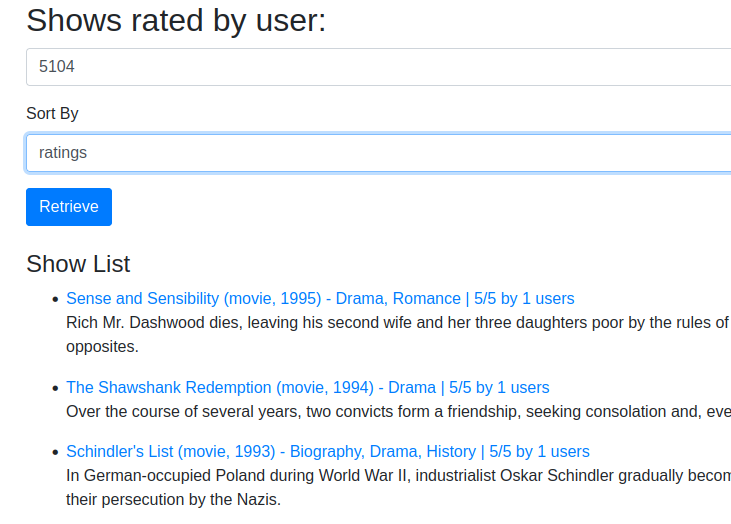
\includegraphics[scale=0.5]{fe1.png}
        \caption{Front End: Screenshot 1}
        \label{fig:fe1}
    \end{figure}
\end{center}

\begin{center}
    \begin{figure}[H]
        \centering
        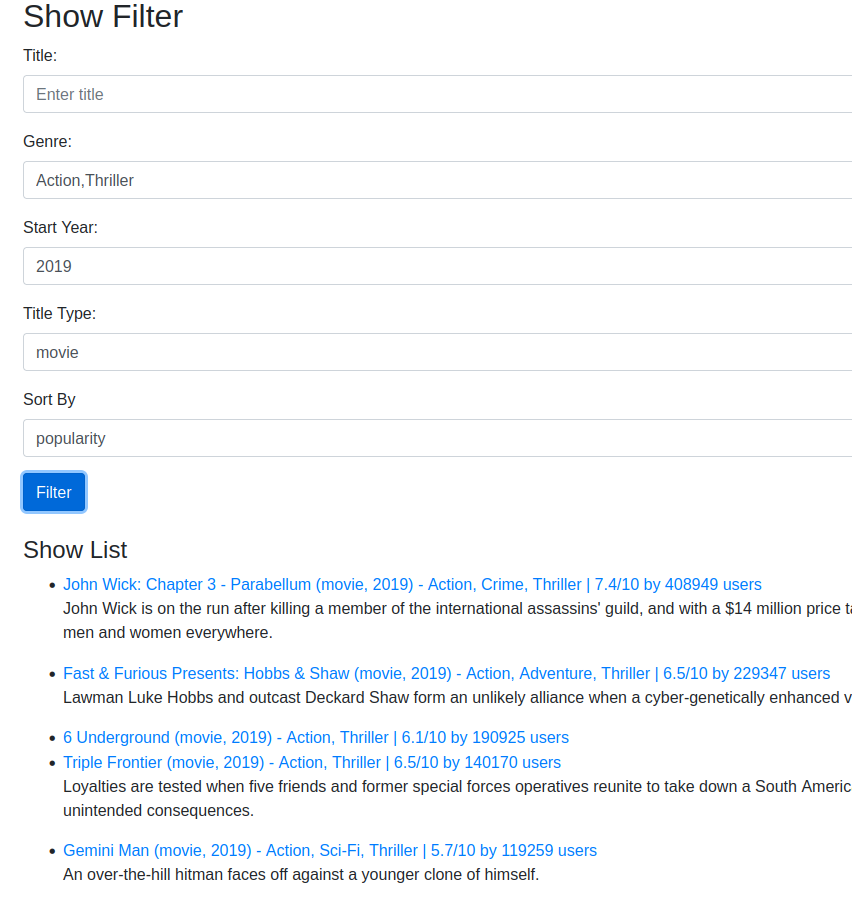
\includegraphics[scale=0.5]{fe2.png}
        \caption{Front End: Screenshot 2}
        \label{fig:fe2}
    \end{figure}
\end{center}

\begin{center}
    \begin{figure}[H]
        \centering
        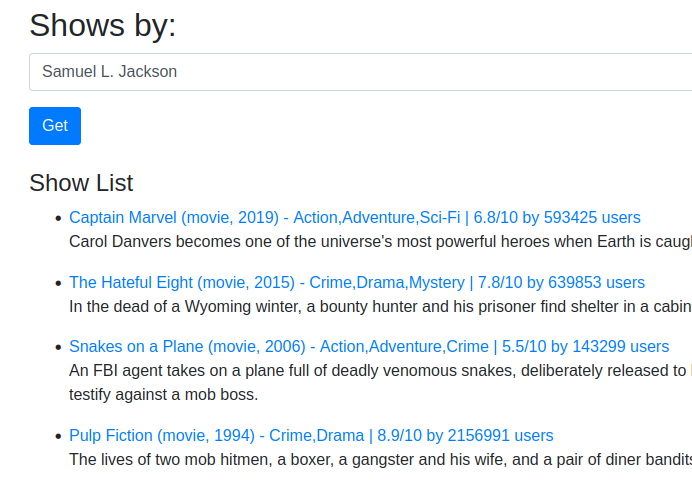
\includegraphics[scale=0.5]{fe3.png}
        \caption{Front End: Screenshot 3}
        \label{fig:fe3}
    \end{figure}
\end{center}

\begin{center}
    \begin{figure}[H]
        \centering
        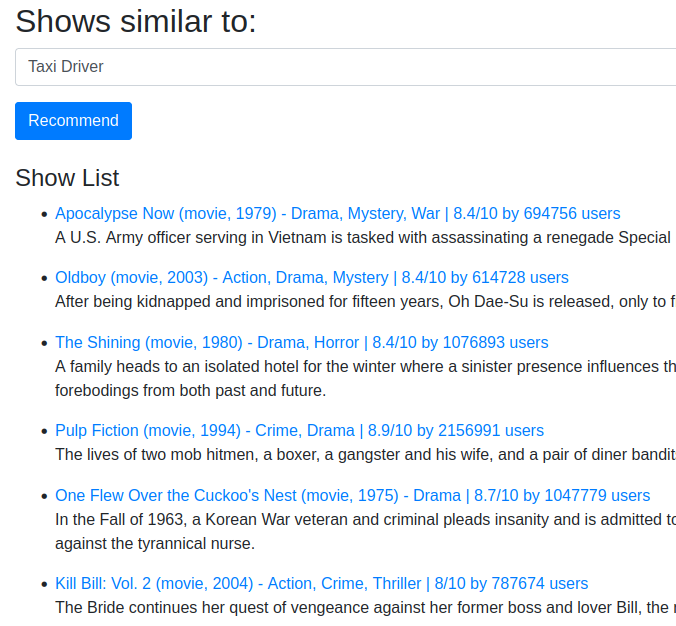
\includegraphics[scale=0.5]{fe4.png}
        \caption{Front End: Screenshot 4}
        \label{fig:fe4}
    \end{figure}
\end{center}


\section{Contribution}

\textbf{Ng Wei Xiang}
\begin{itemize}
    \item Data processing and Cinemagoer dataset 

    \item Neo4j: developed schema, built system, wrote queries, wrote corresponding report section 

    \item Edited and improved all submission items, including codes and schemas
\end{itemize}

\textbf{Rahul Venkatesh}
\begin{itemize}
    \item MongoDB
    \item Frontend
    \item Report formatting (LaTex)
\end{itemize}

\textbf{Wang Yichen}
\begin{itemize}
    \item Data processing
    \item MySQL: developed schema, built system, wrote queries, wrote corresponding report section
\end{itemize}

\textbf{Yong Zhu Cheng}
\begin{itemize}
    \item User event generation
    \item Natural Language queries, MySQL ER diagram
    \item Wrote remaining sections of report. Compiled and edited report for submission.
\end{itemize}

\section{References}

Adams, S. (2022, February 10). How to Join Data in MongoDB. Rockset. https://rockset.com/blog/how-to-join-data-in-mongodb/

GroupLens Research. (n.d.). MovieLens DataSet. https://grouplens.org/datasets/movielens/

Joe Karlsson (2022, January 11). MongoDB Schema Design Best Practices. \\
https://www.mongodb.com/developer/products/mongodb/mongodb-schema-design-best-practices/

Holzschuher, F., Peinl, R. (2013). Performance of graph query languages: Comparison of cypher, gremlin and native access in Neo4j. In Joint EDBT/ICDT 2013 Workshops.

IMDb. (n.d.). IMDb Non-Commercial Dataset. https://developer.imdb.com/non-commercial-datasets/

Khan, W., Ahmad, W., Luo, B., Ahmed, E. (2019). SQL Database with physical database tuning technique and NoSQL graph database comparisons. 2019 IEEE 3rd Information Technology, Networking, Electronic and Automation Control Conference (ITNEC), 110–116. 

Knight, M. (2022, April 26). Graph database vs. document database: Different levels of abstraction. Dataversity. https://www.dataversity.net/graph-database-vs-document-database-different-levels-of-abstraction/ 

Kotiranta P, Junkkari M, Nummenmaa J. (2022) Performance of Graph and Relational Databases in Complex Queries. Applied Sciences. 12(13):6490. https://doi.org/10.3390/app12136490


\end{document}
